\documentclass[a4paper,12pt,twoside]{report}
% \documentclass[a4paper,12pt,twoside]{book}
\pagestyle{headings}
\usepackage[utf8]{inputenc}
\usepackage{filecontents}
\usepackage[many]{tcolorbox}
\usepackage{graphicx}
\usepackage{harpoon}
%\usepackage{apacite} 
\usepackage{xcolor}
\usepackage{latexsym}
\usepackage{amssymb}
\usepackage{amsmath}
\usepackage{mdframed}
%\usepackage[authoryear]{natbib}
\usepackage{hyperref, url}
\usepackage[show]{ed}
\usepackage{subfigure}
\usepackage[ntheorem]{empheq} 
\usepackage{amsthm, amssymb, amsfonts, latexsym}
% \usepackage{pst-all}

\usepackage{enumitem}
\usepackage{multirow}
\usepackage{longtable}
\usepackage[export]{adjustbox}
% $f\arrowvert_A$ To restrict functions

\setlength{\parskip}{1.7em}
\setlength{\parindent}{0em}


%\setlength{\baselineskip}{20pt}

\setlength{\textwidth}{429.75499pt}
\setlength{\textheight}{643.20255pt}
\setlength{\oddsidemargin}{5 mm}
\setlength{\evensidemargin}{5 mm}
\setlength{\topmargin}{0 mm}
\setlength{\headsep}{0 mm}
\setlength{\headheight}{0 mm}


\usepackage{pst-node}

\newcommand{\citealtt}[1]{\citeauthor{#1},\citeyear{#1}}
\newcommand{\myycite}[1]{\citep{#1}}

\mathchardef\mhyphen="2D

%\newcommand{\cev}[1]{\reflectbox{\ensuremath{\vec{\reflectbox{\ensuremath{#1}}}}}}


\usepackage{pst-node,graphicx,pst-blur}
%\uspackage{auto-pst-pdf}
%\usepackage{tikz-cd} 



\makeatletter
\DeclareRobustCommand{\cev}[1]{%
  \mathpalette\do@cev{#1}%
}
\newcommand{\do@cev}[2]{%
  \fix@cev{#1}{+}%
  \reflectbox{$\m@th#1\vec{\reflectbox{$\fix@cev{#1}{-}\m@th#1#2\fix@cev{#1}{+}$}}$}%
  \fix@cev{#1}{-}%
}
\newcommand{\fix@cev}[2]{%
  \ifx#1\displaystyle
    \mkern#20mu
  \else
    \ifx#1\textstyle
      \mkern#20mu
    \else
      \ifx#1\scriptstyle
        \mkern#26mu
      \else
        \mkern#26mu
      \fi
    \fi
  \fi
}

\makeatother

\newcommand{\xcm}{\epsfxsize=3.1cm}
\newcommand{\fig}[1]{\epsfbox}
% \newcommand{\bp}{\begin{minipage}{3.1cm}}
% \newcommand{\ep}{\end{minipage}}



\newtheorem{Definition}{Definition}[]
%\newmdtheoremenv{Theorem}{Theorem}[]
\newtheorem{Theorem}{Theorem}[]
\newtheorem{Lemma}{Lemma}[]
\newtheorem{Proposition}{Proposition}[]
\newtheorem{Corollary}{Corollary}[]
\newtheorem{Remark}{Remark}[]
\newtheorem{Example}{Example}[]


%Shortcut symbols
\newcommand{\Ftheta}{\ensuremath{F_\theta}}


\makeatletter 
\renewcommand{\thefigure}{\@arabic\c@figure}
\makeatother
\usepackage{xr}


%%%% PNAS GRAPHICS SETUP- FROM THE PNAS STYLE LATEX FILE
\RequirePackage{graphicx,xcolor}
\RequirePackage{colortbl}
\RequirePackage{booktabs}
\RequirePackage{algorithm}
\RequirePackage[noend]{algpseudocode}
\RequirePackage{changepage}
\RequirePackage[twoside,%
				letterpaper,includeheadfoot,%
				layoutsize={8.125in,10.875in},%
                layouthoffset=0.1875in,%
                layoutvoffset=0.0625in,%
                left=38.5pt,%
                right=43pt,%
                top=43pt,% 10pt provided by headsep
                bottom=32pt,%
                headheight=0pt,% No Header
                headsep=30pt,%
                footskip=25pt,
                marginparwidth=38pt]{geometry}
\RequirePackage[labelfont={bf,sf},%
                labelsep=period,%
                figurename=Fig. ]{caption}
\setlength{\columnsep}{13.5pt} % Distance between the two columns of text
\setlength{\parindent}{12pt} % Paragraph indent

%% Figure caption style
\DeclareCaptionFormat{pnasformat}{\normalfont\sffamily\fontsize{7}{9}\selectfont#1#2#3}
\captionsetup*{format=pnasformat}

%%% GREYBOX AROUND FIG
\definecolor{lightgray}{gray}{0.95}
\newcommand\greybox[1]{%
  \vskip\baselineskip%
  \par\noindent\colorbox{lightgray}{%
    \begin{minipage}{\textwidth}#1\end{minipage}%
  }%
  \vskip\baselineskip%
}

\newtcolorbox{paperbox}[1][]{
    enhanced,
    colback=white,
    boxrule=0pt,
    boxsep=0pt,
    arc=0mm,
    width=0.8\linewidth,
    fuzzy shadow={0mm}{-4pt}{-4pt}{1mm}{black!30!white},
    #1
}


% \externaldocument{Supp_Koopman-0808}
\begin{document}



\title{Data-Driven Modelling \& \\ Forecasting of Chaotic Systems}



\author{B.L. Nortier} 
\date{January, 2022}
\date{}
\maketitle
% \tableofcontents

% \begin{abstract}
%   Abstract goes here.
%   \end{abstract}

\chapter{Driven Dynamical Systems to Forecast Problems}\label{ch4}

In this chapter, we discuss results pertaining to the mapping of temporal data obtained from a discrete-dynamical system onto a different space through the notion of a driven dynamical system. 
We also consider the conditions a driven system should possess to avoid adding distortion to its state-space representation. We then describe the \emph{single-delay dynamics} (SDD) of the system and and finally recall conditions on the driven system so that the SDD are conjugate (or at least semi-conjugate) to the underlying system. 
The SDD can then be used to forecast and reconstruct the underlying system. 
% \ednote{Is this attractor assumed to exist? M:  I replaced  it with the system. Attractor is also a commonly used term since we observe data from an attractor in almost all cases.}

\section{Nonautonomous and Driven Dynamical Systems}

\begin{Definition}
  [\bf Nonautonomous Dynamical System (adopted from~\cite{Manju_ESP}))] \label{Dfn_NDS}\rm
  A nonautonomous dynamical system (NDS) on a space $X$ is simply a dynamical system comprising a family of maps $\{g_n\}_{n \in \mathbb{Z}}$ where $g_n(\ldotp):=g(u_n,\ldotp):X\to{X}$ is continuous. Each $g_n$ arises as a consequence of an input $u_n$ from the input space $U$, a topological space. 
\end{Definition}

We immediately recall the figure first defined in \eqref{eqn_conjugacy}  and remind ourselves of our ultimate goal to learn a system that is conjugate to an underlying or unknown dynamical system $(U,T)$ by making use of the measurements obtained from  the unknown system.

%#####################################
\begin{center}
\psset{arrows=->, arrowinset=0.25, linewidth=0.6pt, nodesep=3pt, labelsep=2pt, rowsep=0.7cm, colsep = 1.1cm, shortput =tablr}
\everypsbox{\scriptstyle}
\begin{psmatrix}
U & U\\%
V & V.
%%%
%  \ncline{1,1}{1,2}^{T} 
%  \ncline{1,1}{2,1} <{\phi}
%   \ncline{2,1}{2,2}^{S}
%  \ncline{1,2}{2,2} > {\phi}
\end{psmatrix}
%#####################################
\end{center}

To find a function $\phi$, the need now arises to consider a so-called driven dynamical system, a special case of a nonautonomous dynamical system, where two spaces are considered: input is taken from an input space $U$ and the state of a space $X$ is updated. (Previously, only the state was considered.)
We do this to mimic the true conditions. By accounting for both external and internal factors which influence the  system-state at a specific time-step, our model resembles nature much more realistically.  \ednote{M : I understand this sentence, but am not sure if a general audience would. So please elaborate or omit. B: Is this satisfactory?}

\begin{Definition}
  [\bf Driven, Compactly Driven Dynamical System] \label{Dfn_DDS} \rm
A driven dynamical system comprises two topological metric spaces $U$, $X$ and a continuous function  $g:U\times{X}\to{X}$ where $g(u_n, x_n)=x_{n+1}$.
If the input space $U$ is compact, we refer to the system as compactly driven. 
\end{Definition}

The dynamics on X are generated by the update equation $x_{n+1}=g(u_n, x_n)$ where $n\in\mathbb{Z}$, input $u_n$ from $U$ and state $x_n$ belonging to $X$, where $X$ is compact.
Abbreviated, we shall refer only to the \emph{driven system $g$}, with all other entities being understood implicitly.

Notably, a nonautonomous dynamical system may be generated from $U$; any input $\overline{u}$, a bi-infinite sequence from $U$, gives rise to the sequence of self-maps $\{g(u_n, \cdot)\}_{n\in\mathbb{Z}}$ contained in $X$.
Physically, one may think of this bi-infinite sequence as referring to a system that has been running for a long period at the time of the first measurement taken from the system (alternatively, the first time a probe is inserted into the system to take an observation)

\begin{Definition}
  [\bf Entire Solution] \label{Dfn_Soln} \rm
  A sequence $\{x_n\}_{n\in\mathbb{Z}}\subset X$ is called an entire solution (or simply a solution) of the driven system  $g$ with input $\overline{u}$ when it satisfies 
  \[g(u_{n-1}, x_{n-1})=x_n\] for all $n\in\mathbb{Z}$
\end{Definition}

It is important to emphasise that a sequence $\{x_n\}$ satisfying the update equation above can only be a solution if $x_n\in{U}$ holds for all $n\in\mathbb{Z}$ and just for $n>0$. Consider the example below.

\begin{Example} \rm \label{ex_halfux}
  The only solution  $\{x_n\}_{n\in\mathbb{Z}}$ to the driven system  $g(u,x)=\frac{ux}{2}$, where $X=[0,1]$, $U=[0,1]$,  is the zero solution $x_n\equiv0$.
  To see this, consider any $x_n=a\in[0,1]$ where $a\neq{0}$.  Let $\overline{u}\in{U}$ be an non-zero constant sequence , say $u_n=0.5$. 
  The driven system may be rewritten as $x_{n-1}=\frac{2x_n}{u_{n-1}}=4x_n$ and the  iterates of $x_n$ in backward time will increase by a factor of 4 at each timestep. 
  Thus for some $m\leq{n}$,  $1<x_m$ i.e. $x_m\notin{X}$. So ${\{x_n\}}_{n\in\mathbb{Z}}$ is not a solution and it follows that the only possible solution is the zero solution.
\end{Example}
% \ednote{Nicely written!}


A system may also have multiple solutions as is evidenced in the example below.

\begin{Example}\label{Ex_exp} \rm 
 Consider the driven system $g(u_n,x_n)=x^n$ for $X=[0,1]$, $U=\mathbb{R}$. The system has an uncountable number of solutions, as there exists a solution for every $x\in{X}$ which also passes through the point $x$ and $lim_{n\to\infty}x_n=0$, $lim_{n\to{-}\infty}x_n=1$. 
 The proof is deferred to immediately after the next paragraph (see~\ref{rem_proofEx}).
\end{Example}

As the solutions to a driven system are often considered to be an important entity \cite{M: edited the sentence here}, we next identify a subspace $X_U$ of $X$ that contains all possible solutions. To realize such a subspace of a driven system $g$, the concept of a reachable set is defined.

\begin{Definition}
  [\bf Reachable Set]\label{Dfn_ReachableSet}\rm
The reachable set of a driven system $g$ is exactly the union of all the elements of all the (entire) solutions, i.e., 
\[X_U :=\Big \{x \in X:  x = x_k \mbox{ where  $\{x_n\}$  is a solution for some  $\bar{u}$} \Big \}.\]
The set of all reachable states at a specific time $n$ for input $\overline{u}$ is denoted by $X_n(\overline{u})$
\end{Definition}

The reachable set itself can defined independently from the fact that $g$ does or does not have the ESP/USP. We note that $x\in{X_n(\overline{u})}$ if and only $g$ has a solution $\{x_k\}$ for $x_n=x$ and input $\overline{u}$. \textbf{(Cite)}.

$X_n$ is exactly the set of points $x$ through which some entire solution $\Psi$ passes at time $n$.

This will lead to a result established later, but which is worth taking note of now: \textit{$g$ being a topological contraction is equivalent to the existence of a unique entire solution.}

% \begin{Definition}
%   [\bf Topological Contraction]\label{Dfn_TopContr}\rm
%   A function $g:U\times{X}\to{X}$ is a topological contraction if for all $n\in\mathbb{Z}$ and all $\overline{u}\subset{U}$, $X_n(\overline{u})$ is a singleton subset of $X$.  
% \end{Definition}

\begin{Remark}
  [\bf Proof of Example~\ref{Ex_exp}] \label{rem_proofEx} \rm
  To see this, we show that for every input $\overline{u}=\{u_n\}_{n\in\mathbb{Z}}$, $g(u_n,\cdot)$ is a contraction map on $X$ for every $k\in\mathbb{Z}$. 
  Indeed $g(u_n,x_n)=x^n$ depends only on the state at time $n$ and so for each input $\overline{u}$, $X_n(\overline{u})=\{x^n\}$ is a singleton subset.
  We then easily conclude that $\{x_n\}\equiv0$ is the only solution. 
\end{Remark} \ednote{B: Is this sufficient?}

Thus far it has been demonstrated that a system may have one or more solutions; one may ask if a driven system always has a solution and, if so, whether it satisfies certain properties such as uniqueness. 
Should the driven system be compact, existence follows immediately as shown in the following result.

\begin{Theorem}\label{Thm_CompactExistence}
 Let $g$ be a driven system.  If $X$ is compact then for each input $\overline{u}$, there exists at least one solution to the driven system $g(\ldotp, x)$
\end{Theorem}
\begin{proof}
  May be found in \cite{kloeden2011nonautonomous, manjunath2014dynamics, manjunath2013echo}
\end{proof}

One may easily construct many systems with trivial solution-sets, such as $g(u,x)=x$ which has only the constant solution $x$ and so for $U=[-1,1]$, the system would have no solution if $|x|>1$. To refine the scenario, we consider only systems with unique solutions. 

\section{Unique Solution Property}

\begin{Definition}
  [\bf Unique Solution Property] \label{Dfn_usp}\rm
  A driven system $g$ is said to have the Unique Solution Property (USP) if for each input $\overline{u}$ there exists exactly one solution. 
  Alternatively we may formulate the USP as follows: $g$ has the Unique Solution Property if there exists a well-defined map $\Psi:{U}\to{X}$, with $\Psi({\overline{u}})$ denoting the unique solution.
\end{Definition}

One of the first result obtained after defining the USP is the fact that every solution will attract different initial conditions towards the component parts of the solution. %, i.e. that the solution $\Psi$ is a non-autonomous uniform attractor. \ednote{Define Uniform Attractor before stating theorem or else omit the statement.} 
If $g$ has the USP, then any solution to $g$ is also a uniform attractor in nonautonomous dynamical systems literature \cite{Manju_Nonlinearity}. The discussion on nonautonomous attractors is beyond the scope of this project and we refer the reader to \cite{Manju_ESP, esann2012ids} for further reading. 

% \ednote{M: You can omit the theorem, and just say it is a uniform attractor in the nonautonomous dynamical systems literature \cite{Manju_Nonlinearity}, and say the discussion on nonautonomous attractors is beyond the scope of the thesis.}
% Paraphrased.
Additionally, $g$ having the USP is in our context also equivalent to $g$ being a topological contraction \cite{manjunath2021universal}, or alternatively also that $g$ exhibits the Echo State Property (ESP). 

In the majority of Reservoir Computing(RC) literature (a machine learning algorithm approach)\ednote{How should I explain/qualify RC better here? It's mentioned without really explaining.}, 
the ESP is used to describe the concept of fading memory or memory-loss  \cite{jaeger2004harnessing, lu2018attractor}. 
If $g$ possesses the ESP (equivalent in our context to the USP), the we are guaranteed that the whole of an input's left-infinite history will exactly determine the current system state; i.e. there is only ever the possibility of a single reachable state at a given instance of time \cite{jaeger2001echo}

Defined formally, the ESP is intrinsically linked to an input (see \cite{Manju_ESP}) Unfortunately, definitions and results concerning the ESP do not have much practical benefit since a relationship between the network's response and the temporo-statistical properties of the input are not directly described. A more detailed presentation may be found in~\cite{jaeger2001echo}.

We do however consider it important to mention that the ESP is also often discussed in terms of a stability property that holds for all inputs of a system~\cite{manjunath2020stability} and, furthermore, plays a key role in the design and training of recurrent neural networks(RNN) within the field of RC \cite{Manju_ESP}.
 

\section{Next section?}
\ednote{I feel a break is necessary here, but would hear from you what your thoughts are.}

Having already defined the reachable set $X_U$ as the set of all elements of all entire solutions, we pause briefly in order to fix additional notation.
Defining $\cev{u}^{n}:=(\ldots,u_{n-2} ,u_{n-1})$ as the left-infinite subsequence of an input up until time $n$, $\overleftarrow{U}$ is then the notation for all these left-infinite sequences in $U$. 
Moreover, $\cev{u}^{n}v:=(\ldots,u_{n-2} ,u_{n-1}, v)$ will symbolise the input up to time $n$ with $v \in U$ being the specific input value at time $n$. 
The introduction of a new input at time $n$ can be described by the mapping $\sigma_v:   \cev{u}^{n} \mapsto \cev{u}^{n}v$. 
The right-shift map, $r\overleftarrow{U}\to\overleftarrow{U}$, of an input sequence is defined $r: (\cdots, u_{-2},u_{-1}) \mapsto(\cdots, u_{-3},u_{-2})$

The goal now assumes the form of the question on our ability to establish a semi-conjugacy as presented below for the driven system $g$. 
%\ednote{M: I have changed it to a semi-conjugacy since conjugacy amounts to asking a infinite-dimensional space $\overleftarrow{U}$ to be embedded in $X_U$ which is not possible.} 

\begin{equation}  \label{Scomm_h}
  %    \[ 
      \psset{arrows=->, arrowinset=0.25, linewidth=0.6pt, nodesep=3pt, labelsep=2pt, rowsep=0.7cm, colsep = 1.1cm, shortput =tablr}
   \everypsbox{\scriptstyle}
   \begin{psmatrix}
   \overleftarrow{U} & \overleftarrow{U}\\%
   X_U & X_U.
   %%%
  %  \ncline{1,1}{1,2}^{\sigma_v} \ncline{1,1}{2,1} <{h}
  %  \ncline{1,2}{2,2} > {h}
  %  \ncline{2,1}{2,2}^{g(v,\cdot)}
   \end{psmatrix}
  % \]
  \end{equation} 	


We proceed to consider a specific subclass of conjugacies.

  \begin{Definition}
    [\bf Universal Semi-Conjugacy]\label{Def_UnivSemiConj} \rm
    Given a driven system $g$, we  call a continuous and surjective map $h : \overleftarrow{U} \to X_U$ a universal semi-conjugacy if  diagram \ref{Scomm_h} commutes for all $v \in U$.
  \end{Definition}

If the universal semi-conjugacy $h$ exists (i.e. the diagram in \ref{Scomm_h} commutes) then the solution $\Psi$ will be at least a coarse-grained representation of the input $u$. \ednote{B: Expand/Cite}

But does such a function $h$ for the above driven system $g$ above exist? Whenever $g$ has the USP and $\Psi(u)=\{x_n\}_{n\in\mathbb{Z}}$ it follows that $h$, defined by  $h(\cev{u}_n):=g(u_n,x_{n-1})=x_n$, will satisfy the semi-conjugacy in the graph above \ref{Scomm_h}.
Regrettably, such a continuous mapping $h$ is not guaranteed to exist \cite{M: Have edited here} when $g$ does not have the USP \cite[Lemma 5]{Manju_Nonlinearity}.
Note that even when $h$ does exist, we are not guaranteed its injectivity. Considering again example \ref{ex_halfux}, we see that even if $h$ were to exist, it could not be injective as $X_U=\{0\}$.

Re-sketching the commutativity diagram \ref{Scomm_h} above by fixing the input $v$ in $g$ and replacing $X_U$ by its left-infinite sequence space $\overleftarrow{U}$, we obtain the diagram below. In this case, the function $H:\overleftarrow{U}\to\overleftarrow{X}_U$, a map that is both continuous and surjective, is called a \emph{causal mapping}. 

\begin{Definition}
  [\bf Causal Mapping]\label{Def_CausMap}
  A continuous, surjective map $H:\overleftarrow{U}\to\overleftarrow{X}_U$ such that \[H\circ\tilde{g}_v=\sigma\circ{H}\] where $\tilde{g}_v$ maps $(\ldots, u_{-2}, u_{-1})$ to $(\ldots, u_{-2}, u_{-1}, g(v, u_{-1}))$ is called a causal mapping.
\end{Definition}

\begin{equation} \label{SCausal_H}
    %    \[ 
        \psset{arrows=->, arrowinset=0.25, linewidth=0.6pt, nodesep=3pt, labelsep=2pt, rowsep=0.7cm, colsep = 1.1cm, shortput =tablr}
     \everypsbox{\scriptstyle}
     \begin{psmatrix}
     \overleftarrow{U} & \overleftarrow{U}\\%
     \overleftarrow{X}_U & \overleftarrow{X}_U.
     %%%
    %  \ncline{1,1}{1,2}^{\sigma_v} \ncline{1,1}{2,1} <{h}
    %  \ncline{1,2}{2,2} > {h}
    %  \ncline{2,1}{2,2}^{\tilde{g}_v}
     \end{psmatrix}
    % \]
  \end{equation} 	

 \begin{Theorem}
  For a compactly driven system, a causal mapping $H$ exists if and only if $g$ has the USP. 
\end{Theorem}
\begin{proof}
  See~\cite[Th.3]{manjunath2013echo}.
\end{proof}

The driven system $g$ can induce an embedding of $\overleftarrow{U}$ in $\overleftarrow{X}$ as follows: 
If the causal mapping $H:\overleftarrow{U}{\to}{\overleftarrow{X}_U}$ is injective (in addition to being surjective), it becomes the embedding of $\overleftarrow{U}$ in $\overleftarrow{X}$ induced by the driven system $g$. \ednote{Explain why $H_{-1}$ is continuous} and we refer to $H$ as a \emph{causal embedding} 
% \ednote{M : Causal embedding a dynamical system is different from the definition of causal embedding, so please edit/delete this paragraph and the next theorem and also in the remaining part till Section 1.2}. 
% \begin{Theorem}
%  If $g(\ldotp,x)$ is invertible and has the USP then $H$ is a causal embedding. 
% \end{Theorem}
% \begin{proof}
%   See \cite{manjunath2021universal}.
% \end{proof}
When $g$ has the USP, the diagram below (adopted from~\cite{Manju_Nonlinearity}) illustrates the operation of the mappings $h$ and $H$. The mapping $h:\overleftarrow{U}\to{X_U}$ is also considered an observable as mentioned in the introduction of Chapter \ref{ch3}).  

\begin{figure}[ht]
  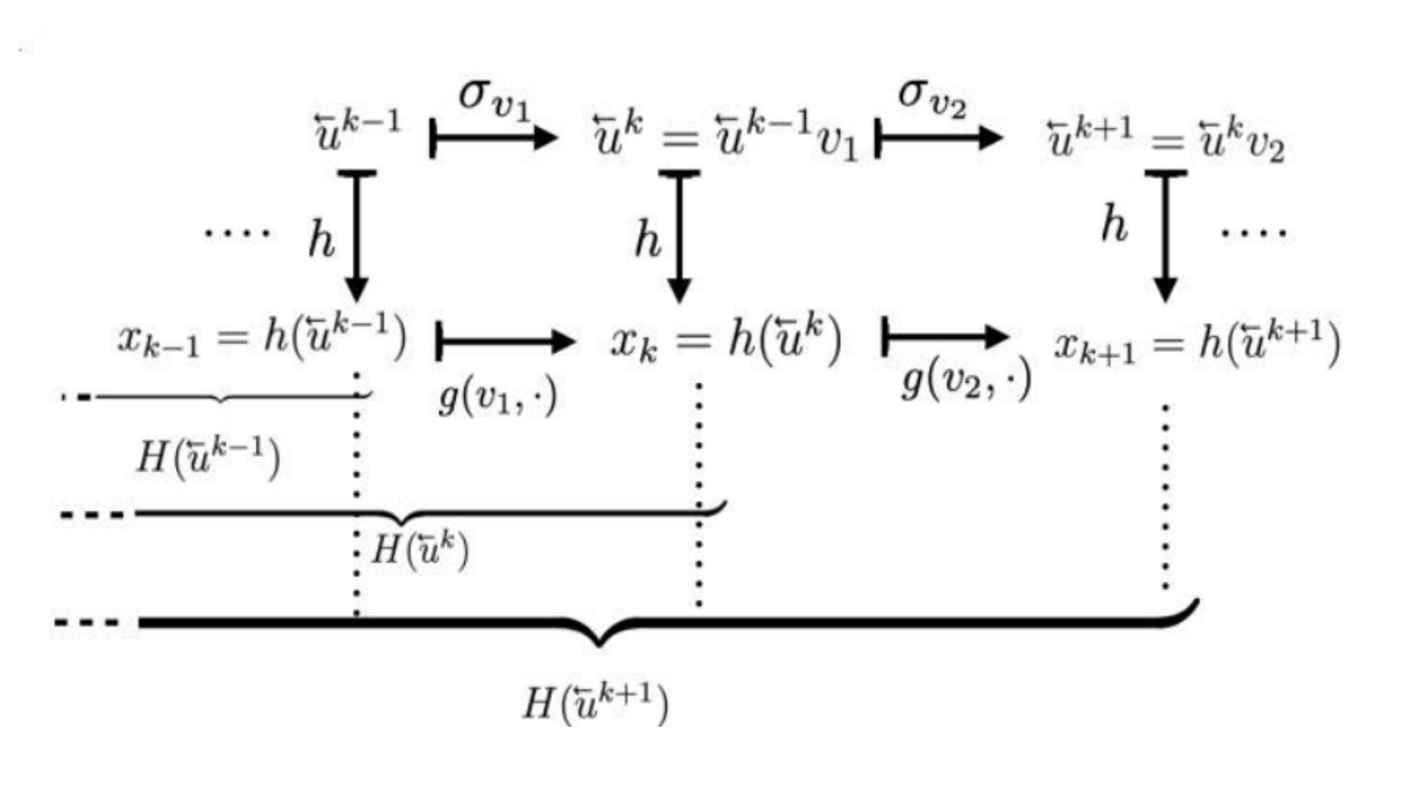
\includegraphics[scale=0.3]{_actionofh_H.eps}
  \centering
  \captionof{figure}{Ladder-like behaviour of $h$ and $H$ to illustrate the causal mapping. }
  \label{fig:actionh_H}
\end{figure}



We wish to explore the possibility of establishing a conjugacy rather than a mere semi-conjugacy and therefore are interested in the restriction of inputs to the left-infinite orbits of a dynamical system.
The left-infinite orbit spaces are significant because a great amount of information about the original system can be gleaned from their topological structure~\cite{Manju_IEEE}. 
The formal topological structure for the so-called inverse-limit space of chaotic dynamical systems is complicated, and further discussion is relegated to~\cite{kennedy2008inverse_limit, ingram2011inverse}.
Broadly, we may conceive of the inverse-limit space of a dynamical system as a self-map on a subset of an infinite-dimensional space where each point in the inverse-limit space corresponds to a backward orbit of the map $T$. 
Following~\cite{manjunath2021universal, ingram2011inverse} we provide a definition:

\begin{Definition}
  [\bf Inverse-Limit Space, Inverse-Limit System]\label{Dfn_InverseL}\rm
 The subset $\widehat{U}_T\subset \overleftarrow{U}$ defined by \[\widehat{U}_T: = \{ (\ldots,u_{-2},u_{-1}): Tu_{i} = u_{i+1}\]is called the inverse-limit space of $(U,T)$.
 The self-map $\widehat{T}$  induced by $T$ on $\widehat{U}_T$  is defined by \[\widehat{T}: (\ldots,u_{-2},u_{-1}) \mapsto  (\ldots,u_{-2},u_{-1},T(u_{-1}))\] and the resulting dynamical system $(\widehat{U_T}, \widehat{T})$ is called the inverse-limit system of $(U,T)$.
\end{Definition}

The inverse-limit space is well-defined since T : U →U is surjective by assumption.


\section{Choosing the driven system $g$}

The driving function $g$ cannot be chosen in a frivolous manner as it could possibly complicate our work. Specifically, one must be careful to avoid a choice of $g$ which would  add complexity to the obtained solution.  

When a causal embedding $H$ exists for the driven system $g$, one can map an arbitrary input ${u}$ onto the solution space $X$ without additional distortion or information-loss \textbf{(Cite.)}.
Established such an embedding eliminates the question of possible additional complexity in the solution by guaranteeing that, since the systems are conjugate (semi-conjugate, \textbf{(refer)}), $g$ does not add any (some) complexity to the system.  

It is, however, a balancing act as it also undesirable to choose a function $g$ that quenches the temporal structure in $u$ by contracting to such a degree that the ability to recover information from the original system is lost completely.
In the above example (\ref{ex_halfux}), the input's temporal variation cannot be related to the reachable set since $X_U$ consists of a single element; little, if not no, information is encoded.
To obtain a suitably complex function $g$, it is thus desired that the reachable set of a driven system  be large enough to relate to the input. 
 We  reguire that the reachable set of a driven system to be such that the inverse-limit space of $U_T$ can be embedded in some finite self-product of the reachable set of $T$ \textbf{(refer or cite)}. To this end, consider the notion of State-Input (SI) Invertibility.  
 \ednote{(M: Expand here. It stops a bit abruptly. B: Does the above reorganisation read better?)} 

\begin{Definition}
  [\bf SI-Invertibility]\label{Dfn_SIinv}\rm
  A map $g$ is said to be SI-Invertible if $g$ is invertible for all $x\in{X}$. Alternatively it may be said that if, given $x_n$ and $x_{n-1}$, $u_{n-1}$ can be uniquely determined from $x_n=g(u_n,x_{n-1})$, then $g$ is said to be SI-invertible.
\end{Definition}
 
SI-invertibility promises that 'enough' information is retained when $g$ is chosen without introducing additional unwanted complexity. \ednote{(M: Expand why this is true. B: Is this satisfactory?)} 
'Enough' here refers to the fact that we may always recover the previous input value $u_n$ (if we know successive states $x_{n-1}, x_n$).
'Without additional complexity' is guaranteed by the invertibility of the function $g$ that guarantees a one-to-one mapping between $u_n, x_{n-1}$ and $x_n$. 
In obtaining an SI-invertible function, therefore, we are guaranteed a system which will not lose so much information about its previous states in the forward-flow of time that one may not make any credible claims as to the original system's behaviour and properties. 
Simultaneously, it does guarantee us that the important information encoded in previous inputs is indeed preserved.

It is worth at this stage taking note of a specific driven system in the form of a discrete state-space model that has acquired some adherence in applications \cite{Manju_IEEE} and especially those pertaining to Echo State Networks and ESP. The function 

\begin{equation}  \label{eqn_driving}
  g(u,x) = (1-a)x + a\overline{\tanh}(Au + \alpha Bx)
\end{equation} 
is both SI-invertible and, if $\alpha\beta<1$, also possesses the USP. 
One may easily show that $g$ is SI-invertible by recovering $u_n$ by 
\begin{equation} \label{eqn_SI_RNN}
  u_{n-1} := A^{-1}\bigg(\overline{\tanh}^{^{-1}}\frac{1}{a}\Big(x_{n+1}-(1-a)x_n\Big) \bigg) - \alpha B x_n
  \end{equation}
  for $x_{n-1}, x_n$ known.

The proof that the map $g$ possesses the USP is rather involved and hence, instead of being replicated here, may be found in \cite[Th.2]{manjunath2013echo }
This specific driving function $g$ is used in our implementation and is discussed more completely in chapter \ref{sect5}

Despite the ease that one may work with a left-infinite history in the realm of theory, it is impossible to obtain such a sequence in any real-life application.  
One does not in practice, fortunately, need the entire left-infinite history of the input thanks to the Uniform Attraction Property (UAP).

\begin{Definition}
  [\bf Uniform Attraction Property]\label{Dfn_UAP}\rm
  A driven system $g$ has the Uniform Attraction Property (UAP) if, regardless of starting position, all trajectories converge to a single trajectory as time flows forward. 
  This trajectory is also the unique solution sequence $x$ to the input sequence $u$ as mentioned above.
\end{Definition}

This definition is stated in a not completely rigourous manner as the more formal definition makes use of processes, a concept which would take some time to establish and detracts from the principal thrust of this project. 
\ednote{B: Is it very obvious to the reader at this point what the general thrust of the paper is?}

As the Unique Attraction Property guarantees that all trajectories will converge to the same trajectory as time moves forward. 
Incredibly, this permits one to initialise a driven system $g$ with an altogether arbitrary initial value $y_m\in{X}$ where $m\in\mathbb{Z}$ and the UAP then guarantees that the sequence $\{y_{m+1}, y_{m+2},\ldots\}$ which satisfies the relation $y_n=g(u_n, y_{n-1})$  for  $k\geq{m}$  will uniformly approach the elements $\{x_n\}$ of the actual solution (See \cite[Th.11,]{Manju_Nonlinearity} or \cite[Eqn.18]{Supp}).
 

\begin{figure}[ht]
  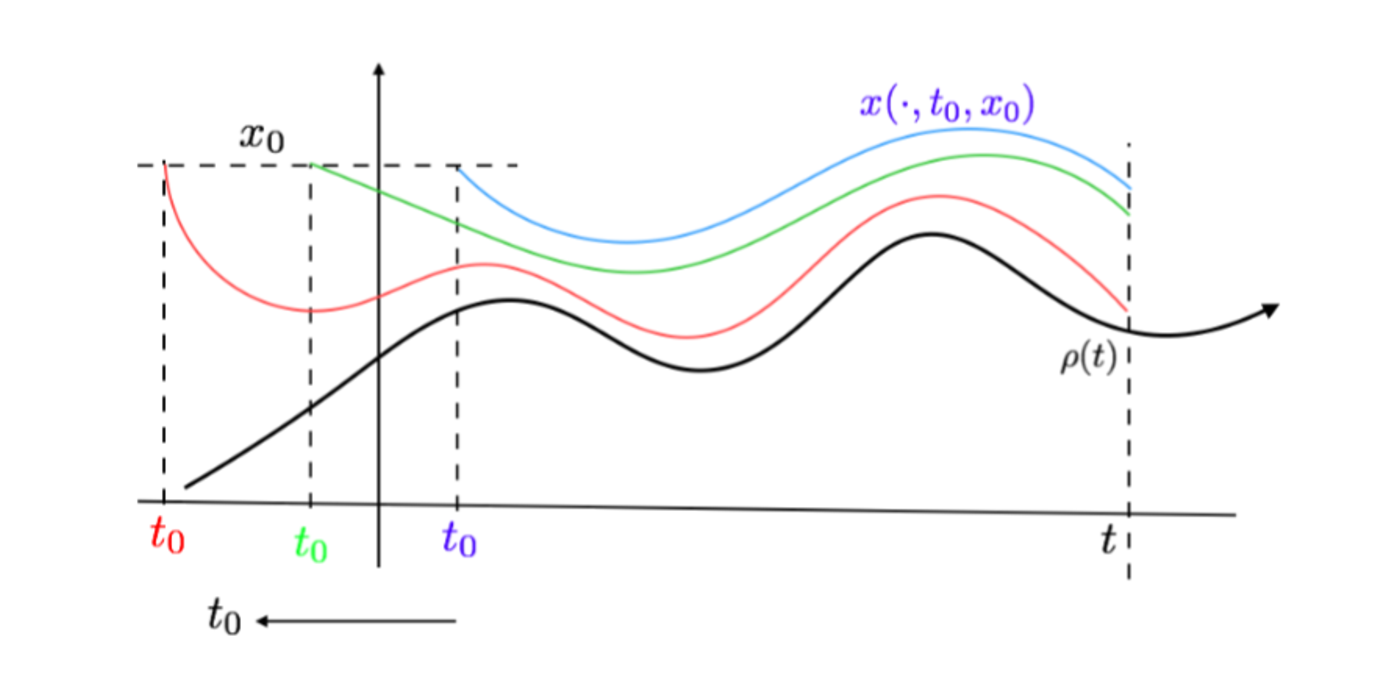
\includegraphics[scale=0.4]{_memloss_conttime.eps}
  \centering
\captionof{figure}{Reproduced from \cite{manunath2021universal}. Illustration of all trajectories approaching the true solution if $g$ has the UAP}
\label{fig:memloss_conttime} 
\end{figure}

One may now appreciate an even more astounding result: $g$ having the USP is equivalent to the UAP. We restate the above theorem.

\begin{Theorem}\label{thm_usp-contr-uap}
  The following statements are equivalent:
  \vspace{-8mm}
  \begin{enumerate}[noitemsep, label=\roman*.]
    \item $g$ has the USP.
    \item $g$ is a topological contraction.
    \item $g$ has the UAP.
  \end{enumerate}
\end{Theorem}
\begin{proof}
  May be found in \cite[Th.1]{Manju_Nonlinearity}
\end{proof}

One need therefore not establish any additional results to ensure that the sequence uniformly approaches the unique solution $\Psi$. This vastly simplifies the effort necessary to set up a problem in order to guarantee that the underlying system will be accurately represented by the conjugate system.

This also solves the problem of perturbation/noise introduced by the observable or measurement function. Recall from before that an observable is inherently a map that discretises the underlying continuous-time system. Moreover, measurement and device error introduce mistakes. Since we are working with a chaotic system displaying sensitive dependence on initial conditions, these small errors could potentially send the trajectory into a completely different attractor. 
In the presence of the UAP, however, small measurement errors introduced into the system do not pose the same danger as before since the trajectories will eventually tend towards the actual solution.
\ednote{(B: Is this Complete enough?)}
% \textbf{From the perspective of perturbation of an autonomous dynamical system, if the resulting nonautonomous system has the USP, then the temporal structure of noise relates to the dynamics on a nonautonomous uniform attractor through a topological semi-conjugacy or a conjugacy.}

\section{The next step in Dynamics}

Next we define the relation $Y_T$ induced by $(U,T)$ on $X_U\times{X_U}$ for a driven system $g$ possessing SI-invertibility.  To describe the  single-delay lag dynamics formally, we consider a dynamical system $T: U \to U$ and we define a relation on the reachable set $X_U$, i.e., a subset defined on $X_U \times X_U$ by 
$$Y_T:=\{(x_{n-1},x_n): \{x_k\}_{k\in \mathbb{Z}} \mbox{ is a solution for some orbit of } T \mbox{ and } n \in \mathbb{Z}\}.$$ 

The following theorem establishes the existence of a well-defined map $G_T$ describing the single-delay dynamics(SDD) of the system above. 

\begin{Theorem}
If we let $G_T:Y_T\to{Y_T}$ be a map defined by the relation $(x_{n-1},x_n)\mapsto(x_n,x_{n-1})$, then $G_T$ is well-defined (and this results holds even in the absence of $g$ possessing over the USP)  
\end{Theorem}

% Recall that $g$ is only being given inputs from the orbits of $T$.  

It is of interest to ascertain whether $\widehat{T}$ and $G_T$ are related\ednote{B: Should I expand more here?}, and we consequently introduce  the function $H_2{\overline{}} := (h(r\overline{u}, h(\overline{u})))$ mapping the entirety of a left-infinite sequence to some element in $X\times{X}$. 
Indeed, it may be shown that $g$ having SI-invertibility and the USP immediately guarantees the existence of at least a semi-conjugacy between the systems $(Y_T, G_T)$ and $(\widehat{U}_T, \widehat{T})$.
This is formalised in Causal Embedding Theorem, which we state next:

\begin{Theorem}
  [\bf Causal Embedding Theorem (adopted from \cite{Supp})]
  % {\bf (Causal Embedding Theorem.)}
 \label{Thm_CET}
	Let $g$ be a driven system with SI-invertibility and the USP. Let $h$ denote the universal semi-conjugacy and $H_2(\overleftarrow{u}) := (h(r\overleftarrow{u}),h(\overleftarrow{u}))$, where $r$ is the right-shift map. 
 Let $(\widehat{U}_T, \widehat{T})$  be the inverse-limit system of a dynamical system $(U,T)$. 
 Then the restriction of $H_2$ to $\widehat{U}_T$ is a topological semi-conjugacy between the inverse-limit system $(\widehat{U}_T, \widehat{T})$ 
and the induced dynamical system  $(Y_T,G_T)$, i.e., the following diagram commutes
\begin{equation} \label{comm_H_CET}
\psset{arrows=->, arrowinset=0.25, linewidth=0.6pt, nodesep=3pt, labelsep=2pt, rowsep=0.7cm, colsep = 1.1cm, shortput =tablr}
 \everypsbox{\scriptstyle}
 \begin{psmatrix}
 \widehat{U}_T & \widehat{U}_T\\%
 Y_T &  Y_T.
 %%%
%  \ncline{1,1}{1,2}^{\widehat{T}} \ncline{1,1}{2,1} <{H_2}
%  \ncline{1,2}{2,2} > {H_2}
%  \ncline{2,1}{2,2}^{G_T}
 \end{psmatrix}
 \end{equation}
or in other words, $(Y_T, G_T)$ is a factor of  $(\widehat{U}_T, \widehat{T})$. Further, if $T:U \to U$ is a homeomorphism, 
then $H_2$ embeds $\widehat{U}_T$ in $X_U \times X_U$, and hence $(Y_T, G_T)$ is conjugate to $(\widehat{U}_T, \widehat{T})$.
\end{Theorem}
\begin{proof}
  May be found as the proof of~\cite[Th.4]{Supp}
\end{proof}

We are drawing nearer and nearer to our principal target and our results carry more and more weight. The next result is remarkable.


\begin{Theorem}
  Graph \ref{Scomm_h} is exactly the inverse-limit system $(\hat{U}, \hat{T})$.    
\end{Theorem}


Recall that $H_2$ maps an entire left-infinite solution sequence from $\Psi$ to an element in $X\times{X}$.
We now have the following (which may be compared with \ref{SCausal_H} above):

\begin{equation} \label{fig:inverse_limsystem}
  %  \[ 
      \psset{arrows=->, arrowinset=0.25, linewidth=0.6pt, nodesep=3pt, labelsep=2pt, rowsep=0.7cm, colsep = 1.1cm, shortput =tablr}
      \everypsbox{\scriptstyle}
      \begin{psmatrix}
      \widehat{U}_T  && \widehat{U}_T \\
      Y_T && Y_T \\
      %%%
     %  \ncline{1,1}{1,2}^{\widehat{T}} \ncline{1,1}{2,1} <{h}
     %  \ncline{1,2}{2,2} > {H_2}
     %  \ncline{2,1}{2,2}^{G_T}
      \end{psmatrix}
    %  \]
  \end{equation}
 

\begin{Theorem}
    $(Y_T, G_T)$ is semi-conjugate to $(\widehat{U}, \widehat{T})$.
\end{Theorem}
\begin{proof}
  See \cite[Th.3, Th.4]{manunath2021universal}
\end{proof}


\section*{Summarising the discussing thus far:}

It is easy to lose the birds-eye view, so we take a moment to review our progress up until this point.

\vspace{-8mm}
\begin{enumerate}
\item We are interested in a some dynamical system $(U,T)$ with unknown dynamics.
\item To determine properties about this system $(U,T)$ and predict its future evolution, we determine the dynamics of the inverse-limit system $(\widehat{U}, \widehat{T})$. Given certain assumptions, we can guarantee that $(\widehat{U}, \widehat{T})$ is at least semi-conjugate to $(U,T)$.
\item If the driven system $g$ is SI-invertible (and $\{u_n\}\in{U}$  is an orbit of $T$), the map $G_T$ exists. 
\item If, furthermore, $g$ has the USP, $(Y_T, G_T)$ is semi-conjugate to $(\widehat{U}, \widehat{T})$.
\item If we can assume that $T$ is a homeomorphism, $(Y_T, G_T)$ is topologically conjugate to $(\widehat{U}, \widehat{T})$, an extension space of $(U,T)$
\end{enumerate} 

One can therefore learn the SDD of the driven system states via $G_T$ with enough data thanks to the USP/UAP. This enables us to do at least two things: 
\vspace{-8mm}
\begin{itemize}
\item Forecast future values of $x_n$ via iterates of $G_T$ (as $G_T$ can be determined.
\item Forecast future values of $u_n$. 
\end{itemize} 

% Below is reproduced a pictorial representation of the relationship between different entities and properties. \textbf{(Cite SIG_25May)}
% Below is reproduced a pictorial representation of the relationship between the different entities and their properties.

\begin{figure}[ht]
  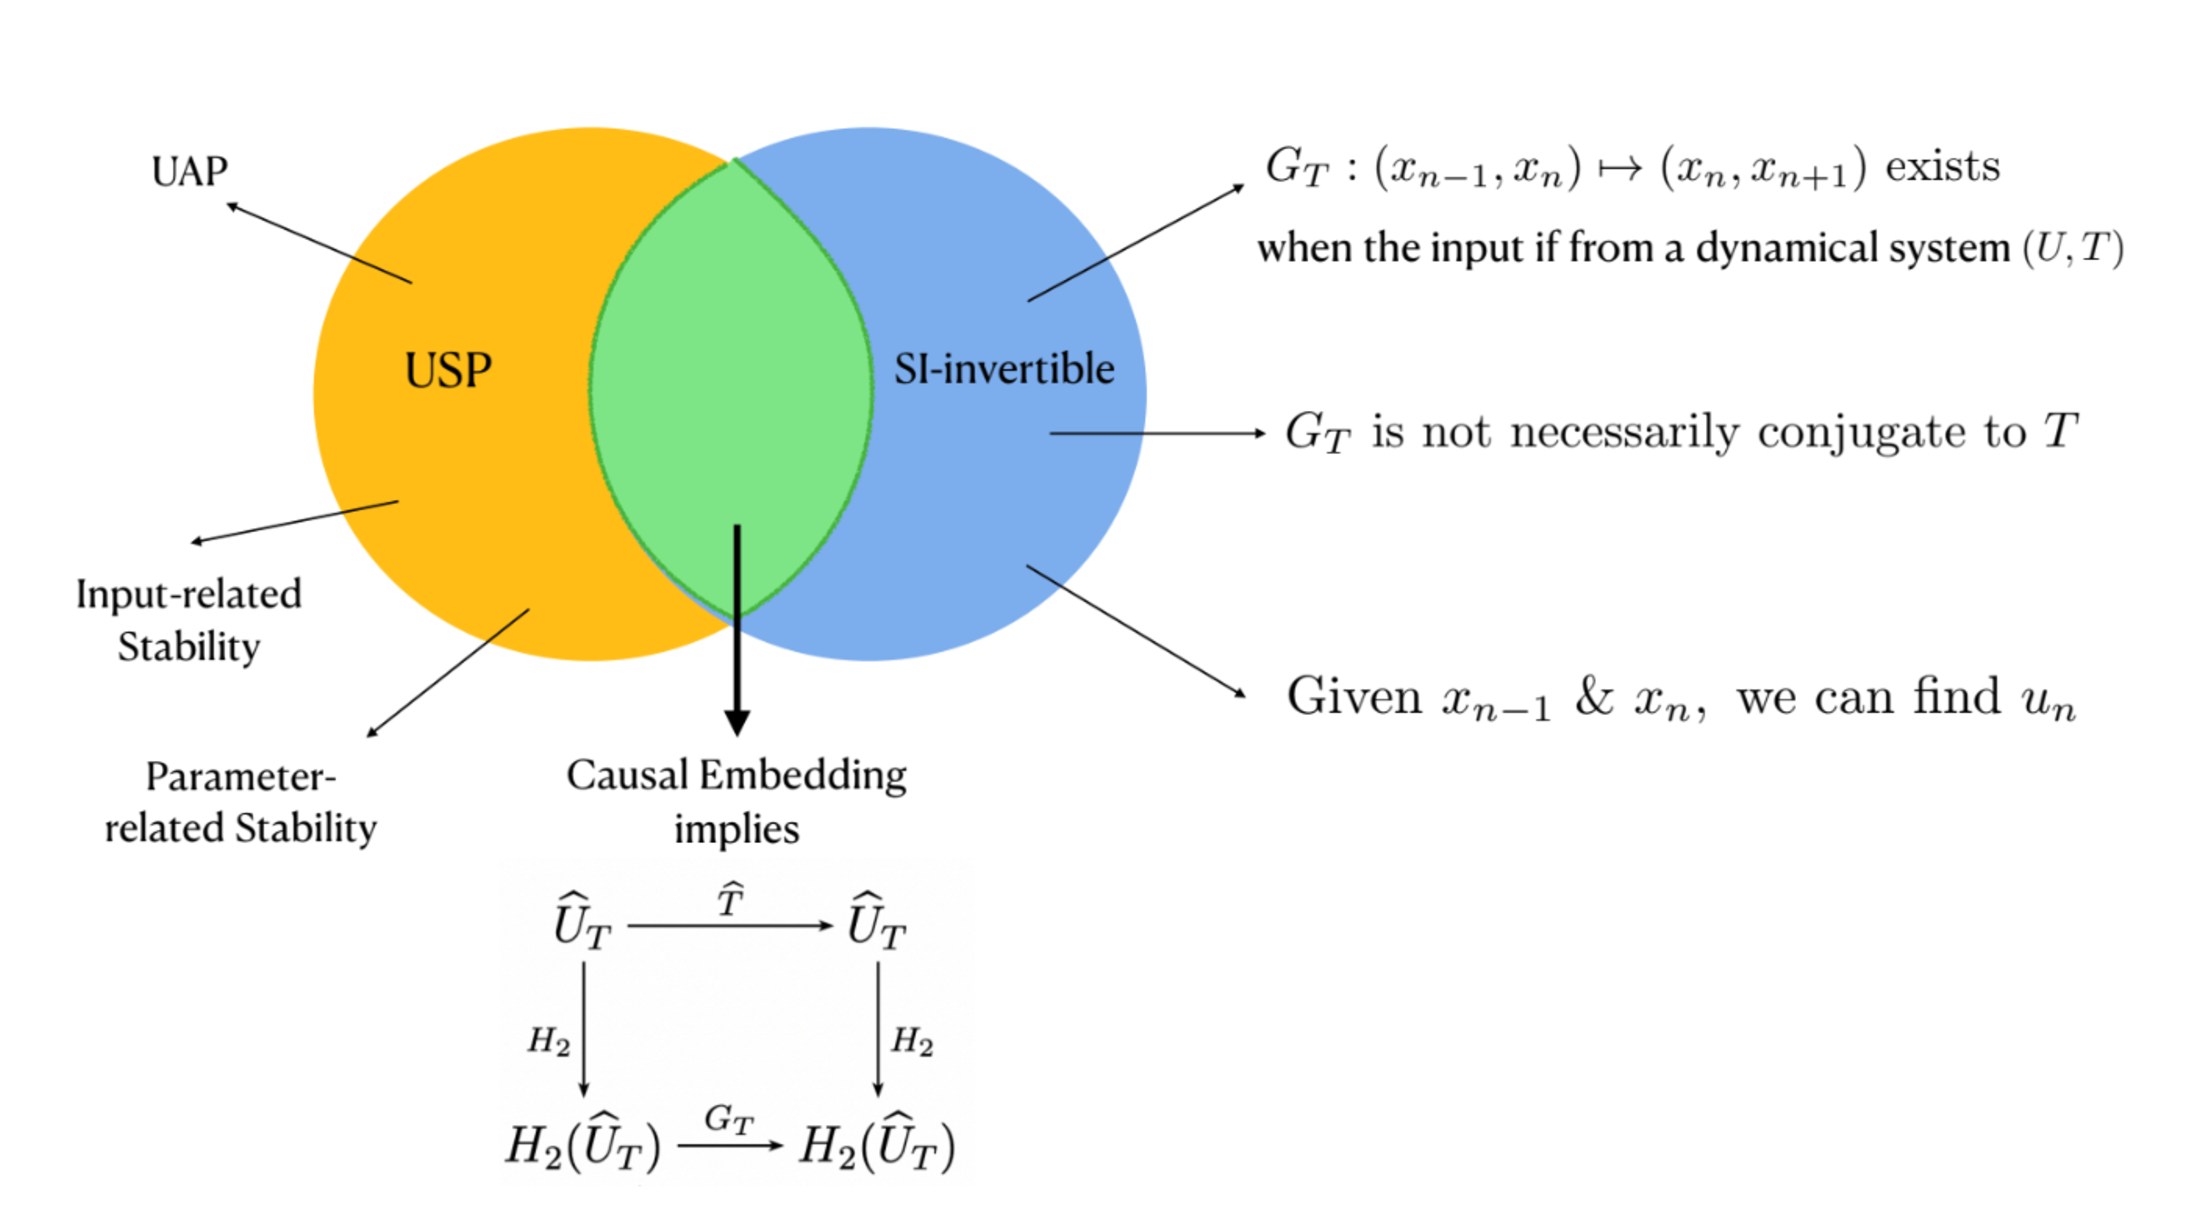
\includegraphics[scale=0.3]{_summarypictorial.eps}
  \centering
  \label{fig:fig_pictorialSummary}
\end{figure}



\end{document}